\chapter{引言}

\section{RNA-Seq}
\nocite{wang2009rna, ozsolak2010rna}

RNA-Seq 是对 RNA 序列进行测量的一种技术, 
它是近几年来发展起来的通过深度测序用于研究转录组的一种技术. 
与其他的方法相比起来, RNA-Seq 揭露了生物的转录组中更多的复杂性. 
同时, RNA-Seq 能够更好地研究生物的转录组中各转录本的表达量. 
通过了解细胞中在某种特定条件下转录组中的转录本的组成, 
以及每一个转录本的表达量, 我们可以了解基因上的不同的功能模块, 
进而了解生物的发育过程, 以及疾病与人体之间的关系. 
通过使用 RNA-Seq, 我们已经对编码蛋白质的基因以及它们的剪切异构体 (isoform) 有了更为深入的了解. 
此外, RNA-Seq 也帮助我们对于基因上的非编码区域有了更为深入的认识, 
例如 lncRNA (long non-coding RNA).
并且我们对 sRNA (small RNA), microRNA 等也有了更全面的了解. 
\cite{pickrell2010understanding, encode, nagalakshmi2008transcriptional, 
tang2009mrna, banfai2012long, mortazavi2008mapping, wang2008alternative, 
katz2010analysis, deng2011isoform, lu2010function, mercer2011targeted, 
howald2012combining, lalonde2011rna, djebali2012landscape, 
derrien2012gencode, gerstein2012architecture, fairfax2012genetics, 
morrissy2011extensive, howald2012combining, park2012rna, 
tilgner2012deep, orom2010long, mercer2011human, chung2011computational, 
gingeras2009implications, roy2010identification, axtell2011vive, 
berezikov2010evolutionary, cherbas2011transcriptional, anders2012detecting, 
stoeckius2009large, lau2009abundant}

在 RNA-Seq 技术出现之前, 人们主要通过微阵列 (microarray) 对转录组进行定量分析和研究 \cite{schena1995quantitative}. 
但是与 RNA-Seq 相比, 微阵列存在若干问题 \cite{wang2009rna}: 
\begin{itemize}
\item 微阵列只能在序列已知的情况下使用

\item 结果会受交叉杂交 (cross-hybridization) 影响 \cite{okoniewski2006hybridization, royce2007toward}

\item 测量的表达量范围有限
\end{itemize}
另外, 在 RNA-Seq 技术出现之前, 人们主要通过 Sanger 测序法对互补 DNA (cDNA) 序列或者表达序列标签库 (EST libraries) 进行测序来研究转录组的序列 \cite{boguski1994gene, gerhard2004status}. 
但是 Sanger 测序价格昂贵, 同时测序通量偏低, 无法对转录组进行定量分析和研究. 
高通量测序技术的发展使得我们能够在较短的时间内用较少的成本对大量序列进行测序, 
几乎完整地测量转录组的序列, 
同时建立测序数量和实际被测序分子的数量间的关系 \cite{marioni2008rna}. 
这些是 RNA-Seq 在当今被广泛应用的一个主要原因. 

\begin{figure}[!t]
\centering
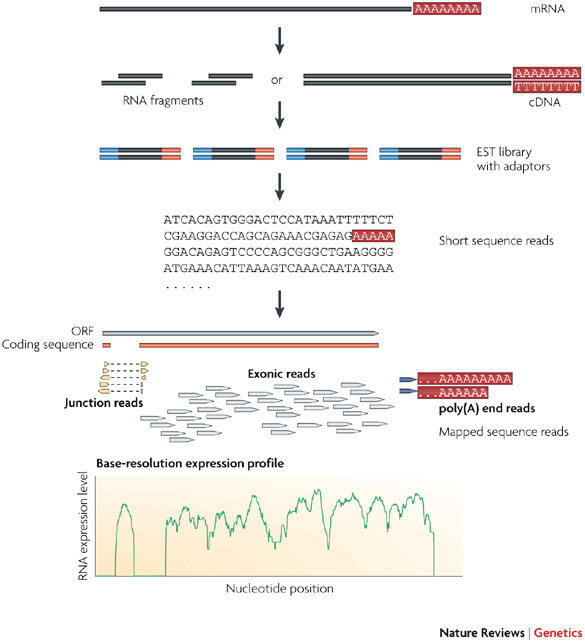
\includegraphics[width=\textwidth]{figures/rna-seq-experiment.jpg}
\caption{一般的 RNA-Seq 实验流程 \cite{wang2009rna}}
\label{intro-rna-seq-ex}
\end{figure}

\section{RNA-Seq 数据分析方法简介}
RNA-Seq 通常直接用于对于这些生物问题的研究:
\begin{itemize}
\item 发现新的剪切异构体 \cite{merkin2012evolutionary, wang2010novo, roberts2011identification, wang2010mapsplice}

\item 研究 RNA 序列的对于生物的调控作用 \cite{van2011xuts}

\item 比较不同条件下转录组不同的构成 \cite{trapnell2012differential}
\end{itemize}
同时, RNA-Seq 数据还未研究其他生物问题提供了宝贵的原始数据, 
例如对于生物系统中的网络的研究 \cite{sinicropi2012whole}. 

为了能够通过 RNA-Seq 数据对生物问题有深入的研究, 
我们通常会对 RNA-Seq 数据用这些方法进行处理:
\begin{itemize}
\item 序列比对 (sequence alignment): 将 RNA-Seq 读段找到其在基因组中的位置

\item 序列拼装: 
直接将 RNA-Seq 读段拼装成原转录组的各转录本. 若拼装时不依赖已知的参考序列, 
则成为 \textit{de novo} 拼装 ((\textit{de novo} assembly)). 

\item 转录本的表达量估计: 用一定的单位表示每个被测样本中转录组里每个转录本的含量, 
用于在不同的样本之间进行比较

\item 辨识同一个基因的剪切异构体 (真核生物 RNA-Seq 数据): 真核生物中由于选择性剪切同一个基因会产生多个剪切异构体, 
通过 RNA-Seq 数据在一定条件下可以辨识出一个基因的不同的剪切异构体
\end{itemize}

\subsection{序列比对}
经典的序列比对算法包括 Smith-Waterman 算法 \cite{SmithWaterman1981} 和 Needleman-Wunsch 算法 \cite{needleman1970general}. 
但是由于 Smith-Waterman 算法和 Needleman-Wunsch 算法复杂度偏高, 它们不适用于大规模的数据. 
目前人们一般采用一些启发式的方法进行序列比对 \cite{isaev2004introduction}. 
对于将 RNA-Seq 读段比对到其在基因组中的位置, 目前比较常用的工具包括: 
\begin{itemize}
\item BLAT \cite{kent2002blat}
\item TopHat \cite{trapnell2009tophat}
\end{itemize}

\subsection{序列拼装}
序列拼装是生物信息学和计算生物学中一个经典的问题, 
其目的是通过测序的读段恢复出原始的生物序列. 对于序列拼装, 目前人们主要采用一下这两种常用的策略: 
\begin{itemize}
\item OLC (overlap-layout-consensus) \cite{greenphrap, bonfield1995new, 
kececioglu1995combinatorial, myers1995toward, huang1999cap3}

\item de Bruijn 图 \cite{pevzner2001eulerian}
\end{itemize}
目前对于 RNA-Seq 数据的拼装主要有这些常用的工具: 
\begin{itemize}
\item Cufflinks \cite{cufflinks.2010}: 
OLC 策略 (图 \ref{intro-cufflinks-assembly})

\item Trinity \cite{grabherr2011full}: 
de Bruijn 图策略 (图 \ref{intro-trinity-assembly})
\end{itemize}

\begin{figure}[!t]
\centering
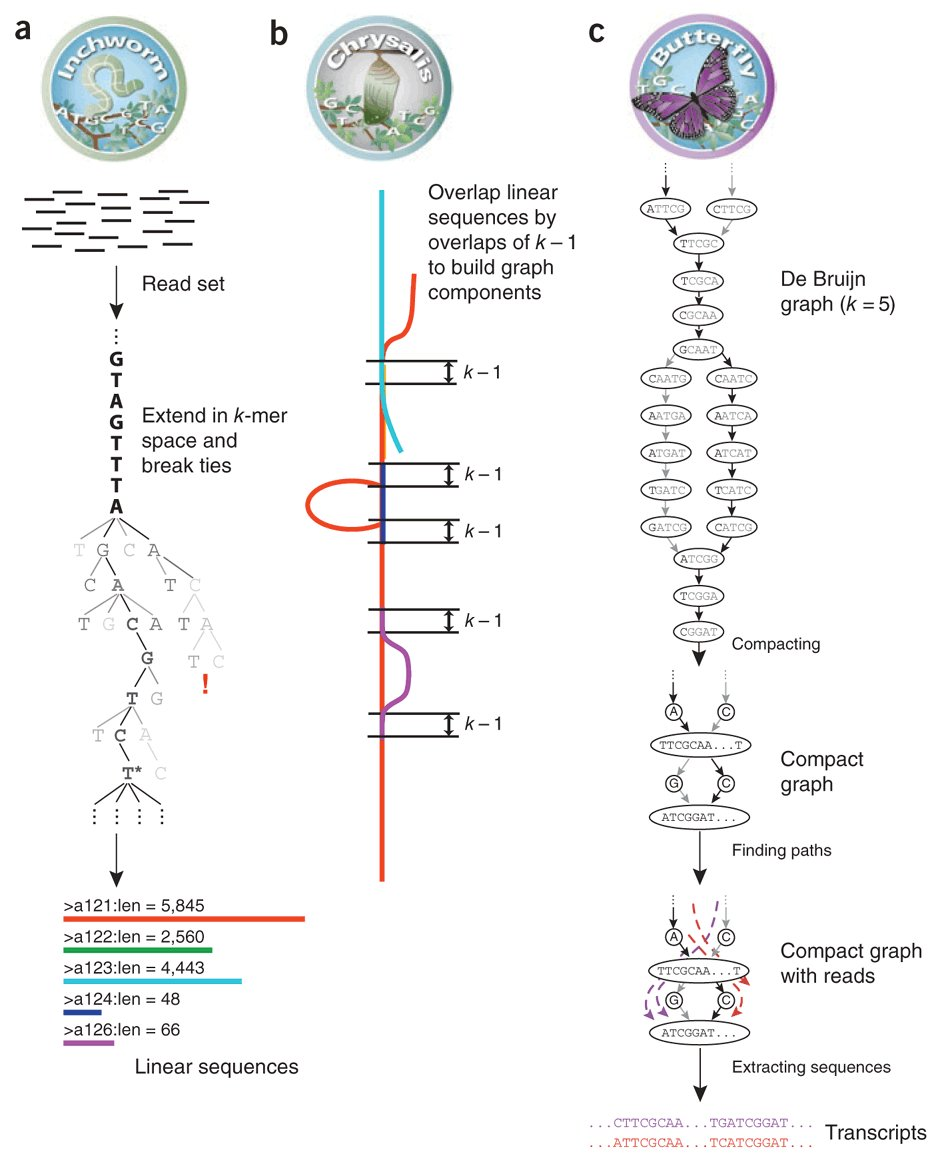
\includegraphics[width=\textwidth]{figures/trinity-assembly.jpg}
\caption{Trinity 拼装策略 \cite{grabherr2011full}}
\label{intro-trinity-assembly}
\end{figure}

\subsection{转录本的表达量估计}
通过量化转录组中各转录本, 从实验数据中估计其表达量, 
我们可以对生物系统中的结构和过程有更好的量化的认识. 
RNA-Seq 技术的发展对于转录本表达量的估计有很大的帮助. 
在 RNA-Seq 实验中, 
通常使用 RPKM (reads per kilobase per million reads sequenced) 
\cite{mortazavi2008mapping} 作为一个转录本表达量的单位. 
目前在 RNA-Seq 实验中通常使用的转录本表达量估计的工具包括: 
\begin{itemize}
\item Cufflinks \cite{cufflinks.2010} (图 \ref{intro-cufflinks-abundance})
\end{itemize}

\begin{figure}[!t]
\centering
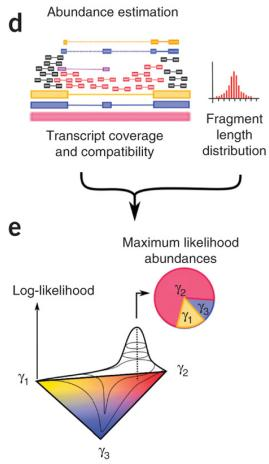
\includegraphics[height=0.5\textheight]{figures/cufflinks-abundance.jpg}
\caption{Cufflinks 对转录本的表达量的估计 \cite{cufflinks.2010}}
\label{intro-cufflinks-abundance}
\end{figure}

\subsection{辨识同一个基因的剪切异构体 (真核生物 RNA-Seq 数据)}
经过多年的研究, 人们认识到真核生物的同一个基因会有多个剪切异构体 
\cite{gilbert1978genes, rosenfeld1982calcitonin, early1980two, 
citeulike:447573, modrek2002genomic}. 
RNA-Seq 技术的发展大大促进了人们对于真核生物中选择性剪切的认识, 
因为 RNA-Seq 数据可以较好地表现出来真核生物中的选择性剪切的现象. 
目前在真核生物相关的 RNA-Seq 实验中通常使用的用于辨识同一个基因的剪切异构体的工具包括: 
\begin{itemize}
\item Cufflinks \cite{cufflinks.2010} (图 \ref{intro-cufflinks-assembly})
\end{itemize}

\begin{figure}[!t]
\centering
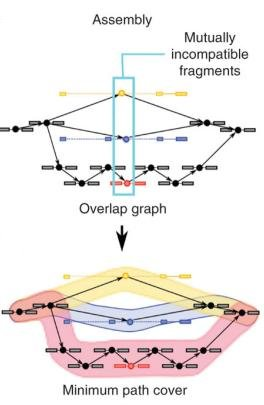
\includegraphics[height=0.5\textheight]{figures/cufflinks-assembly.jpg}
\caption{Cufflinks 序列拼装策略和对同一个基因的剪切异构体的辨识 \cite{cufflinks.2010}}
\label{intro-cufflinks-assembly}
\end{figure}

\section{现有基于 RNA-Seq 数据的转录本表达量估计和剪切异构体辨识方法}

\subsection{RNA-Seq 数据定量分析的一般模型}
\label{rna-seq-general-model}

\onlinecite{2011arXiv1104.3889P} 对RNA-Seq 数据定量分析建立了一个一般的模型, 
用统计的方法对 RNA-Seq 数据进行定量分析. 在这里我们对这个模型进行介绍. 

下面是为了描述该模型所使用的一些符号, 以及一些假设: 
\begin{itemize}
\item $G$ 表示转录组中所有包含的基因所组成的集合. 

\item 所有读段构成的集合表示为 $R$, 同时所有的读段都是单端测序得到的等长读段. 
(对于双端测序数据以及不等长读段的数据的处理与这里的模型相似, 此处为了叙述简便不再赘述, 
有兴趣的读者可参考 \onlinecite{cufflinks.2010, 2011arXiv1104.3889P}.)

\item $I_g$, $g \in G$ 表示基因 $g$ 在转录组中所有的剪切异构体组成的集合, 
$I = \bigcup_{g \in G} I_g$ 是所有的剪切异构体所构成的集合. 
此处为了方便描述, 我们也将无选择性剪切的基因所对应的转录本称作是它的剪切异构体. 

\item $\theta_i \geq 0$, $i \in I$ 是剪切异构体 $i$ 的表达量, 
它们满足 $\sum_{i \in I} \theta_i = 1$. 记 $\theta_I = {\theta_i | i \in I}$.
在该模型下, 此处定义的表达量和实际中 RPKM 表达的表达量成正比 \cite{cufflinks.2010}. 

\item $q(p, i)$ 表示对于一个剪切异构体 $i \in I$, 
来自 $i$ 的一个读段的起始位置 (5' 段) 是 $p$ 的概率. 
对于给定的一个剪切异构体 $i$, 
$\sum_{p \in \{ \text{所有读段起始位置} \}} q(p, i) = 1$. 
对于处理实际 RNA-Seq 数据中遇到的读段分布不均匀的问题我们可以通过调整 $q(p,i)$ 
以改进方法的准确性 \cite{roberts2011improving}. 

\item 当给定一个剪切异构体 $i$ 和它上面一个读段的起始位置 $p$ 时, 
$q(p, i)$ 是已知的. 

\item 一个读段 $r \in R$ 可以是来自多个 $I$ 中的剪切异构体, 
但是给定一个剪切异构体 $i$, 
用序列比对的方法将 $r$ 比对到 $i$ 上的所有位置是唯一的. 
(对于基因序列的分析表明这样一个假设是合理的 \cite{peng2011t}.) 

\item 对于一个读段 $r$ 和一个剪切异构体 $i$, 定义 $a_{ri}$: 
\[
a_{ri} = \begin{cases}
0 & \text{当 $r$ 不能比对到 $i$ 上时} \\
q(\text{$r$ 比对到 $i$ 上的起始位置},i) & \text{当 $r$ 能比对到 $i$ 上时} \end{cases}
\]

\item 对于每一个读段 $r \in R$, 
都存在一个剪切异构体 $i \in I$ 使得 $r$ 是可以由 $i$ 产生的一个读段. 

\item 所有的读段都是独立的. 
\end{itemize}

由以上我们可以得到观察到所有读段 $R$ 的似然函数: 
\begin{equation}
\label{rna-seq-general-likelihood}
L(R) = \prod_{r \in R} (\sum_{i \in I} a_{ri} \theta_i)
\end{equation}

\subsection{转录本表达量估计和剪切异构体辨识}
在已知所有剪切异构体的集合 $I$ 时, 通过式 \eqref{rna-seq-general-likelihood} 中的似然函数, 
我们可以对各剪切异构体的表达量进行估计. 
Cufflinks 是在 RNA-Seq 实验中一个常用的工具 (图 \ref{intro-cufflinks-assembly}). 

当我们不知道剪切异构体的集合 $I$ 时, 
我们可以通过过优化通过式 \eqref{rna-seq-general-likelihood} 中的似然函数, 
或者其他的目标函数, 在进行剪切异构体集合 $I$ 的辨识的同时对各转录本的表达量进行估计. 
已发表的方法包括: 
\begin{itemize}
\item NSMAP \cite{nsmap.21575225}

\item IsoLasso \cite{isolasso.recomb}

\item CEM \cite{Li15112012}

\item iReckon \cite{Mezlini29112012}

\item SLIDE \cite{Li13122011}

\item Montebello \cite{Hiller.Montebello}
\end{itemize}

下面我们对若干已发表的通过 RNA-Seq 数据进行转录本表达量估计和剪切异构体辨识的工具进行介绍. 

\subsubsection{Cufflinks}
Cufflinks 对于剪切异构体的辨识和转录本表达量的估计如图 \ref{intro-cufflinks-assembly} 
和图 \ref{intro-cufflinks-abundance} 所示. 
Cufflinks 是分开处理剪切异构体的辨识和转录本表达量的估计这两个流程的. 
对于剪切异构体的辨识, Cufflinks 在 读段所构成的剪切图 
(splicing graph) \cite{Heber01072002} 寻找一个最小的路径覆盖, 
但是 Cufflinks 并不是直接在剪切图上进行操作的. 
Cufflinks 通过在读段之间定义一个序, 
并且在这个序构成的二分图上计算最小花费最大匹配来构成所求的最小路径覆盖. 
在定义该二分图各边的权重时, Cufflinks 采用了 \onlinecite{wang2008alternative} 
的方法启发式地定义权重. 

\subsubsection{NSMAP, CEM, iReckon, 和 Montebello}
NSMAP, CEM, iReckon, 和 Montebello 这 4 个工具是同时进行剪切异构体的辨识和转录本表达量的估计的. 
由于一个基因可能的剪切异构体的个数相当的多, NSMAP, CEM, 和 Montebello 
采用了带惩罚项的似然函数进行剪切异构体的辨识和转录本表达量的估计. 
其具体做法是对式 \eqref{rna-seq-general-likelihood} 中的似然函数增加一个惩罚项, 
变为求剪切异构体的集合 $I$ 和它们的表达量 $\theta_I$ 使得
\begin{equation}
e^{-\Phi} L(R) = 
e^{-\Phi}\prod_{r \in R} (\sum_{i \in I} a_{ri} \theta_i)
\end{equation}
最大化, 其中 $\Phi$ 是一个惩罚项, 其中使用以下这些方法等: 
\begin{itemize}
\item Lasso \cite{tibshirani1996regression}: 
$\Phi = \lambda \sum_{i \in I} |\theta_i|$, $\lambda > 0$ 

\item BIC \cite{BIC.Schwarz_1978}: 
$\Phi = \frac{|I|}{2} \log |R|$
\end{itemize}

\subsubsection{IsoLasso 和 SLIDE}














